\documentclass[11pt,oneside]{article}
\usepackage{enumitem, hyperref}
\usepackage[margin=0.5in]{geometry}
\usepackage{graphicx}
\graphicspath{ {images/} }

% \newcommand{\localCommand}[1]{\texttt{\\ \\ user@localhost: #1\\ \\ }}

\newcommand{\localCommand}[1]{\begin{quote} \texttt{user@localhost: #1} \end{quote}}
\newcommand{\remoteCommandBeforeRename}[1]{\begin{quote} \texttt{pi@raspberrypi: #1} \end{quote}}
\newcommand{\remoteCommandAfterRename}[1]{\begin{quote} \texttt{pi@pulse000: #1} \end{quote}}

\newcommand{\remoteCommandAfterRenameTiny}[1]{\begin{quote} \texttt{\tiny pi@pulse000: #1} \end{quote}}

\newcommand{\myurl}[1]{\begin{quote} \texttt{#1} \end{quote}}
\newcommand{\scriptline}[1]{\begin{quote}$\!\!\!\!\!\!\!\!\!\!\!\!\!$ \texttt{#1} \end{quote}}
\newcommand{\xtermOutput}[1]{\begin{quote} \texttt{>\$ #1} \end{quote}}
\newcommand{\xtermPartialOutput}[1]{\begin{verse} \texttt{#1} \end{verse}}

% \newcommand{\xtermPartialOutput}[1]{\begin{quote} \texttt{#1} \end{quote}}

\newcommand{\eatNewline}{\vspace{-22.0pt}}

\pagenumbering{gobble}  % TURN OFF PAGE NUMBERING

\title{Raspberry Pi Preparation}

\author{Phoebe J. Welch}

\begin{document}
\maketitle

\section*{Introduction}
This document describes how to configure a RaspberryPi so that it will:
\begin{itemize}
	\item Allow remote access from a trusted remote computer without requesting credentials.
	\item Function without keyboard, mouse, monitor.
	\item Run programs written in Python-2, Python-3 and Java-9.
	\item Boot from a USB thumb drive rather than a MicroSD card.
\end{itemize}
\subsection*{Conventions/Assumptions}
\begin{itemize}
	\item Host machine is a Mac running OS X.  This machine will be referred to as the {\em local host}.
	\item Raspberry Pi will be configured to run the Raspbian Stretch Lite OS.  The Pi will be referred to as the {\em remote host} or
	{\em target host} or {\em target machine}.
	\item Local host can be connected to the target machine with ethernet cable.
	\item Commands to be issued on the local host will have the following format: \localCommand{local-host-command}
	\item Commands to be issued on the remote host will have two different formats.  Before the hostname of the remote host is changed
	from the default (raspberrypi) commands will have the following format: \remoteCommandBeforeRename{remote-host-command}  After
	the hostname of the remote host is changed (this document uses the name pulse000), commands will have the following format:
	\remoteCommandAfterRename{remote-host-command}
	\item Output that appears in an XTerm will have the following format: \xtermOutput{this is output on the command line in an xterm}
	\item URLs appear as: \myurl{http://www.some.url.com}
	\item It is assumed that the reader knows how to use vi.
	\item If this document becomes a standard reference, Item \ref{itm:copyBashAliases} of Section \ref{sect:configureRaspberryPi} will need to be updated,
	and all of Section \ref{sect:raspberryPiAccessInternet} will need to be updated.
\end{itemize}

\section{Get The Required Software} \label{sect:getRequiredSoftware}
\begin{enumerate}
	\item Download SD Card Formatter
	\myurl{https://www.sdcard.org/downloads/formatter\_4/}
	We will use this to format the SD Card with the initial image of the Raspbian operating system.  We will use this for
	the initial boot of the Pi.  Later we will configure the Pi to boot from a USB thumb drive.
	\item Download Etcher
	\myurl{https://etcher.io}
	We will use this to format the USB thumb drive with the initial image of the Raspbian operating system.  This will be our boot drive.
	\item \label{itm:getRaspbian} Download \& install Raspbian Stretch Lite.  Don't get Raspbian with Desktop,
	you won't be hooking a monitor up to the Pi so you don't need it.
	\myurl{https://www.raspberrypi.org/downloads/raspbian/}
	You should get a file that's called something like: \xtermPartialOutput{2017-11-29-raspbian-stretch-lite.img}
\end{enumerate}

\section{Prepare the MicroSD Card} \label{sect:prepareMicroSDCard}
\begin{enumerate}
	\item Attach the MicroSD card to the Mac.
	\item \label{itm:msdFormat} Open the SD Card Formatter.  Select Overwrite Format.
	\item \label{itm:msdDoFormat} Click on Format (this will take a while).
	\item When format has finished check that the SD card appears in Finder.  It should be under \texttt{Devices} and it should be called \texttt{BOOT}.
	\item \label{itm:msdEtcher} Open Etcher, push Select Image and find the Raspbian \texttt{.img} file you downloaded at step \ref{itm:getRaspbian} of Section
	\ref{sect:getRequiredSoftware}.  This will write the Raspian operating system to the MicroSD Card.
	\item \label{itm:msdDoEtcher} Push Flash and wait for MicroSD card to be imaged.
	\item \label{itm:diskutilMicroSD} Open a terminal window and run
	\localCommand{diskutil list}
	You want to figure out where the MicroSD card is mounted, so look for \xtermPartialOutput{FDisk\_partition\_scheme 32.0GB}  You should see something like this:\\
	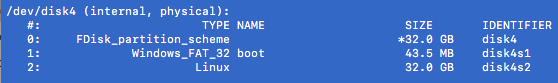
\includegraphics[scale=0.9]{diskutil1.png}\\
	So, given this, we know the MicroSD card is located at \texttt{/dev/disk4}.
	\item \label{itm:unmountMicroSD} Unmount the MicroSD card:
	\localCommand{diskutil unmountDisk /dev/disk4}
	(Note: replace \texttt{/dev/disk4} with what we saw when we ran the \texttt{diskutil list} command in step \ref{itm:diskutilMicroSD}).
	\item \label{itm:removeMicroSD} Remove the MicroSD card.
\end{enumerate}

\section{Prepare the USB Thumb Drive}
\begin{enumerate}
	\item Attach the USB card to the Mac.  It should appear in the Finder as \texttt{NO NAME}.  Use the SD Card Formatter to format \texttt{NO NAME} as we did for the MicroSD card
	in items \ref{itm:msdFormat} and \ref{itm:msdDoFormat} of Section \ref{sect:prepareMicroSDCard}.  Again, this will take a while.
	\item Check that \texttt{NO NAME} appears in the Finder under \texttt{Devices}.
	\item Open Etcher and, as we did in items \ref{itm:msdEtcher} and \ref{itm:msdDoEtcher} of Section \ref{sect:prepareMicroSDCard}, select the Raspbian \texttt{.img} file and push Flash
	to write the Raspbian operating system to the USB Thumb Drive.
	\item Repeat steps in items \ref{itm:diskutilMicroSD}, \ref{itm:unmountMicroSD} and \ref{itm:removeMicroSD} of Section \ref{sect:prepareMicroSDCard} to unmount \& remove the USB
	Thumb Drive.
\end{enumerate}

\section{Enable SSH on Remote Host}
We do this so that we can log into the RaspberryPi remotely.  If we did not do this we'd need to attach a monitor, keyboard \& mouse to the RaspberryPi.
\begin{enumerate}
	\item \label{itm:insertSSHRH} Insert the MicroSD card into the host machine.  It should appear in Finder (for some reason it was now called \texttt{boot}, {\em lower case}, when I
	went through this process; YMMV\footnote{Your Mileage May Vary, a common acronym among programmers.}.)
	\item \label{itm:cdSSHRH} Change directory into the MicroSD card: \localCommand{cd /Volumes/boot}
	\item \label{itm:createSSHSSHRH} Create an empty file called \texttt{ssh} on the MicroSD card: \localCommand{touch ssh}
	\item \label{itm:cdHomeSSHRH} Return to your home directory: \localCommand{cd}
	\item \label{itm:ejectSSHRH} Eject the MicroSD Card (\texttt{boot}) from the Finder.
	\item \label{itm:removeSSHRH} Remove the MicroSD card.
	\item Repeat steps \ref{itm:insertSSHRH} through \ref{itm:removeSSHRH} for the USB Thumb Drive.
\end{enumerate}

\section{Boot Up the RaspberryPi from the MicroSD Card} \label{sect:bootRPIFromMSD}
\begin{enumerate}
	\item Insert the MicroSD card into the RaspberryPi
	\item Connect the network cable to the host machine and to the RaspberryPi
	\item Power up the RaspberryPi
	\item \label{itm:pingPISSDCard} Wait for a while, then confirm that the RaspberryPi is up, running and networked to the host machine.  The network name of the RaspberryPi
	is \texttt{raspberrypi.local} so ping it to see if it responds: \localCommand{ping raspberrypi.local}
	You should see something like:
	\xtermPartialOutput{64 bytes from 169.254.18.127: icmp\_seq=1 ttl=64 time=0.436 ms}
	If you do then everything's good.  Note that in this case the IP address of the RaspberryPi is \texttt{169.254.18.127}; you might want to make a note of this.
	\item Log into the RaspberryPi remote host: \localCommand{ssh pi@raspberrypi.local}
	This will give you some scary-looking warning about the authenticity of the host not being established.  Don't worry, just type 'yes' at the prompt.  The password is \texttt{raspberry}.
	At this point the remote host will suggest that you change the password.  This is a good idea, but don't do it now (we change the password in section \ref{sect:configureRaspberryPi},
	step \ref{itm:changePWD}).  You're now logged into the RaspberryPi!
\end{enumerate}

\section{Configure the Pi to be Bootable from the USB Thumb Drive} \label{sect:thumbBootConfigure}
This section and sections \ref{sect:thumbBootConfirm} and \ref{sect:thumbBoot} are optional but highly recommended.  Booting from a USB Thumb Drive is faster than booting from a MicroSD card
and will improve the reliability of the Raspberry Pi system. If you decide to continue booting from the MicroSD card skip to section \ref{sect:raspberryPiAccessInternet}.
\begin{enumerate}
	\item On the remote host, open the \texttt{/boot/config.txt} file for editing: \remoteCommandBeforeRename{sudo vi /boot/config.txt}
	\item At the bottom of the \texttt{/boot/config.txt} file, add the following lines: \xtermPartialOutput{\# Enable boot from USB Drive\\ program\_usb\_boot\_mode=1}
	\item Save \& exit vi.
	\item Insert USB Thumb Drive into any of the USB slots.
\end{enumerate}

\section{Reboot and Confirm Configuration} \label{sect:thumbBootConfirm}
\begin{enumerate}
	\item In the terminal window for the RaspberryPi: \remoteCommandBeforeRename{sudo reboot}
	The connection to the remote host will be closed.  Wait for a bit....
	\item Ping the remote host again: \remoteCommandBeforeRename{ping raspberrypi.local}
	If you see stuff like: \xtermPartialOutput{64 bytes from 169.254.18.127: icmp\_seq=0 ttl=64 time=0.387 ms} it means the remote host is back up \& running.
	\item Log into remote host again: \localCommand{ssh pi@raspberrypi.local}
	The password is still \texttt{raspberry}
	\item On the remote host, run: \remoteCommandBeforeRename{vcgencmd otp\_dump | grep 17}
	You should see: \xtermPartialOutput{17:3020000a}
	If you do it means that the RaspberryPi is now configured to boot from the USB Thumb Drive.
\end{enumerate}

\section{Boot from the USB Thumb Drive} \label{sect:thumbBoot}
\begin{enumerate}
	\item Shut down the remote host: \remoteCommandBeforeRename{sudo halt}
	Wait for a bit, then power off the remote host.
	\item Remove the MicroSD Card, leave the USB Thumb Drive.
	\item Power up the RaspberryPi (and keep your fingers crossed).
	The first time the RaspberryPi is booted from the thumb drive it will take a long time to come up.  Don't worry, after the first boot from USB Thumb Drive the startup time will be greatly reduced.
	\item Ping the RaspberryPi to confirm it's back up.  If ping is unsuccessful do not worry, just wait a little longer and try again.
\end{enumerate}

\section{Configure RaspberryPi to Access Internet} \label{sect:raspberryPiAccessInternet}
The steps required to configure the RaspberryPi to access the internet depend upon the facilities available.  Filling in the details of this step is TBD.
After this is done remember to disconnect the ethernet cable from the host computer and the Pi.

\section{Configure the RaspberryPi} \label{sect:configureRaspberryPi}
\begin{enumerate}
	\item Log into remote host: \localCommand{ssh pi@raspberrypi.local}
	The password is still \texttt{raspberry} but we will soon change that.  Note that you may get a long, confusing error about \texttt{ECDSA host key and DNS SPOOFING} and you won't be able to log in.
	To fix this, on your local machine: \localCommand{vi ~/.ssh/known\_hosts} and look for \texttt{raspberrypi.local}.  This {\em SHOULD} be the last line or $2^{nd}$-to-last-line of the file.
	Delete this line.  It's possible the RaspberryPi's IP address also made it into this file.  If it did, delete that line, too.  Recall that the IP address was found in Step \ref{itm:pingPISSDCard}
	of Section \ref{sect:bootRPIFromMSD}.
	\item Enter the command: \remoteCommandBeforeRename{sudo raspi-config}
	You will see a crude GUI that looks like this:\\
	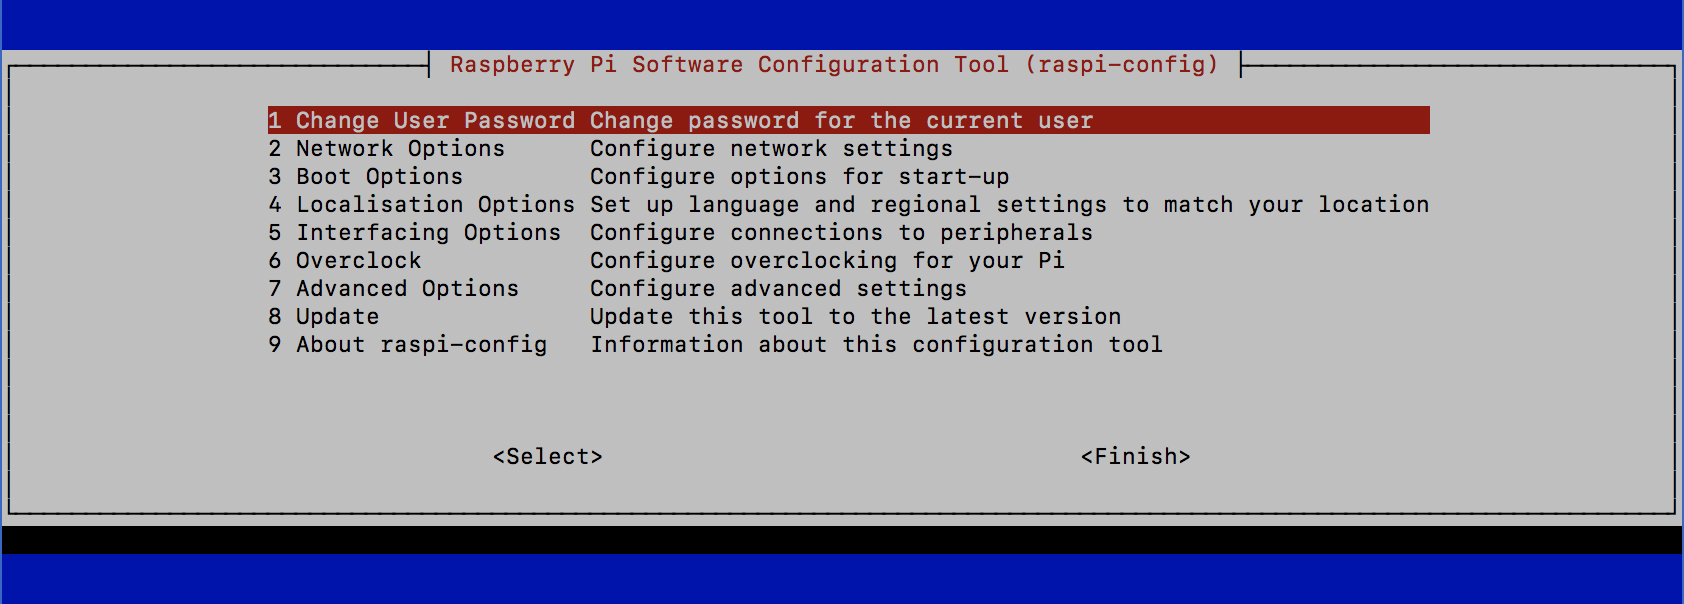
\includegraphics[scale=0.6]{raspiconfig.png}\\
	Use the arrow keys to navigate, hit ENTER to select.
	\begin{enumerate}
		\item Select \texttt{Change User Password} and follow the instructions.  Please be sure to remember the password, and {\em don't} make it too easy to guess. \label{itm:changePWD}
		\item Select \texttt{Network Options}, then select \texttt{N1 Hostname} and follow the instructions to change the network name of the RaspberryPi.  For this project I recommend
		changing it to something like \texttt{pulse000} (you never know when you might need 1000 networked RaspberryPis to get your project working).  Henceforth we will assume the
		name of the RaspberryPi is \texttt{pulse000.local}
	\end{enumerate}
	\item Exit out of \texttt{raspi-config} by selecting \texttt{Finish}.  Confirm that the changes took effect by entering the command: \remoteCommandAfterRename{hostname}
	You should see the network name you gave to the RaspberryPi.
	\item Exit out of the RaspberryPi, then log back in: \localCommand{ssh pi@pulse000.local}
	Be sure to enter your new password.  If you logged in successfully then everything's groovy.
	\item \label{itm:copyBashAliases} Copy the \texttt{bash\_aliases} file in \texttt{{\textasciitilde}/Dropbox/RaspberryPi} to \texttt{/home/pi/.bash\_aliases} on 
	the remote host RaspberryPi (note the leading '.' in the target file's name).
	This is a small file (only two lines), but we'll be adding to it so it makes sense to copy it to the RaspberryPi now.
	\localCommand{scp {\textasciitilde}/Dropbox/RaspberryPi/bash\_aliases pi@pulse000.local:.bash\_aliases}
	Enter your password when prompted.  If you \texttt{ssh} into \texttt{pulse000.local} as \texttt{pi} and type the command: \remoteCommandAfterRename{ll .bash\_aliases} you should see something
	like: \xtermOutput{-rw-r--r-- 1 pi pi 42 Mar 10 20:37 .bash\_aliases}
	Now that you're logged into the RaspberryPi, you might as well create a subdirectory of \texttt{/home/pi} called \texttt{.ssh} \remoteCommandAfterRename{cd; mkdir .ssh}
	This will be useful in Section \ref{sect:configureWorkWithoutPassword},
	when we configure the local machine and the remote RaspberryPi so that \texttt{ssh} and \texttt{scp} will not prompt for a password.
\end{enumerate}


\section{Configure \texttt{ssh} and \texttt{scp} to Work Without Password} \label{sect:configureWorkWithoutPassword}
This section assumes the host machine is running Mac OS X.  Windows/Linux systems will require a different procedure.
\begin{enumerate}
	\item \label{itm:genIdRsa} Make sure that the files \texttt{id\_rsa} and \texttt{id\_rsa.pub} do not already exist in \texttt{{\textasciitilde}/.ssh} on the local machine
	(note: if the \texttt{{\textasciitilde}/.ssh} directory
	does not exist just go to Item \ref{itm:sshkeygen} below).  If the \texttt{.ssh} directory and the \texttt{id\_rsa} and \texttt{id\_rsa.pub} files {\em do} exist, just rename the two files to something else.
	\item \label{itm:sshkeygen} Run the following command from your home directory on the local host: \localCommand{ssh-keygen -t rsa}
	Accept the defaults, don't enter a passphrase.
	\item \texttt{cd} into \texttt{{\textasciitilde}/.ssh} and confirm that the files \texttt{id\_rsa} and \texttt{id\_rsa.pub} were generated.  Use \texttt{scp} to copy \texttt{id\_rsa.pub} to the
	\texttt{/home/pi/.ssh} directory you created in Item \ref{itm:copyBashAliases} of Section \ref{sect:configureRaspberryPi}: \localCommand{scp id\_rsa.pub pi@pulse000.local:/home/pi/.ssh/id\_rsa.pub}
	\item Log into the RaspberryPi with ssh and \texttt{cd} to \texttt{.ssh} directory.  Confirm that the \texttt{id\_rsa.pub} file is in this directory.  Because this is the first time you've set up this
	RaspberryPi to accept \texttt{ssh} and \texttt{scp} without password there should be no file named \texttt{authorized\_keys} in this directory, but just to be on the safe side confirm this.  If no such
	file exists then it's OK to rename the file \texttt{id\_rsa.pub} to \texttt{authorized\_keys}: \remoteCommandAfterRename{mv id\_rsa.pub authorized\_keys}
	However, if you want to configure a second local host so that it can \texttt{ssh} without password to this RaspberryPi, it is important that you {\em append} the contents of \texttt{id\_rsa.pub}
	to the existing \texttt{authorized\_keys} file.  To do this, use \texttt{vi} to add a blank line to the end of \texttt{authorized\_keys}, then: \remoteCommandAfterRename{cat id\_rsa.pub >> authorized\_keys}
	After you've done this, get rid of \texttt{id\_rsa.pub}: \remoteCommandAfterRename{rm id\_rsa.pub}
	\item On the local host machine, make sure that \texttt{ssh-agent} is running: \localCommand{ps auxwww | grep ssh-agent}
	and look for something like\footnote{If you {\em don't} see this, I'm not sure what to do.}: \xtermPartialOutput{user               4275   0.0  0.0  4297428   5068   ??  S     5:00PM   0:00.04 /usr/bin/ssh-agent -l}
	\item Add the private key to the \texttt{ssh-agent} by running: \localCommand{ssh-add -K {\textasciitilde}/.ssh/id\_rsa}
	\item Rename the files you generated in Item \ref{itm:genIdRsa}: \localCommand{mv id\_rsa pulse000\_id\_rsa ; mv id\_rsa.pub pulse000\_id\_rsa.pub}
	If you named your RaspberryPi something other than \texttt{pulse000} then change the above commands accordingly.
	\item Look for a file called \texttt{config} in the local host's \texttt{{\textasciitilde}/.ssh} directory.  If it does not exist, use \texttt{vi} to create it and perform Items \ref{itm:defaultForAll} and \ref{itm:hostPulse000}
	below.  If it does exist it may be OK to skip Item \ref{itm:defaultForAll} but definitely perform Item \ref{itm:hostPulse000}.
	\begin{enumerate}
		\item \label{itm:defaultForAll} Add the following lines to the top of the \texttt{config} file: \xtermPartialOutput{\#\#\# default for all \#\#\# \\Host *\\ \ AddKeysToAgent yes \\ \ UseKeychain yes}
		\item \label{itm:hostPulse000} Add the following lines to the end of the \texttt{config} file:
		\xtermPartialOutput{\#\#\# override for pulse **\\ Host pulse000\\ \ HostName pulse000.local\\ \ User pi\\ \ IdentityFile {\textasciitilde}/.ssh/pulse000\_id\_rsa}
	\end{enumerate}
	\item To test that this worked, on local host run the following: \localCommand{ssh pulse000}
	This should log you into the RaspberryPi as user pi {\em without} prompting for a password.
\end{enumerate}

\section{Update the Raspbian Operating System, Install/Update the JDK, Get Packages}
\begin{enumerate}
	\item Log into remote host: \localCommand{ssh pulse000}
	No password required (but don't forget the password!)
	\item Update the Operating System: \remoteCommandAfterRename{sudo apt-get update -y \&\& sudo apt-get upgrade -y}
	\item Install Java.  It is only possible to install one version of Java at a time so perform either \ref{itm:InstallJava8} {\em or} \ref{itm:InstallJava9}, below, {\em but not both}.
	\begin{enumerate}
		\item Java 8: \label{itm:InstallJava8}
		\begin{enumerate}
			\item Get Java 8 from Oracle \& install: \remoteCommandAfterRename{sudo apt-get update \&\& sudo apt-get install oracle-java8-jdk}  This
			will take a while.
			\item Confirm installation: \remoteCommandAfterRename{java -version}  As of \today\ this should return: \xtermPartialOutput{java version "1.8.0\_65"}
		\end{enumerate}
		\item Java 9\footnote{This information was obtained from \myurl{https://www.raspberrypi.org/forums/viewtopic.php?t=200232}}: \label{itm:InstallJava9}
		\begin{enumerate}
			\item Add the repo to \texttt{/etc/apt/sources.list}: \remoteCommandAfterRename{sudo vi /etc/apt/sources.list}  Add the following 
			line to the end of that file: \xtermPartialOutput{deb http://ftp.de.debian.org/debian stretch-backports main}
			\item Get Java 9 \& install: \remoteCommandAfterRename{sudo apt-get update \&\& sudo apt-get install openjdk-9-jdk-headless}
			\item Confirm installation: \remoteCommandAfterRename{java -version}  As of \today\ this should return: \xtermPartialOutput{openjdk version "9-Raspbian"}
		\end{enumerate}
	\end{enumerate}
	\item Get Git: \remoteCommandAfterRename{sudo apt-get install git}
	Answer 'Y' when asked if you want to continue.
	\item Get python setup tools: \remoteCommandAfterRename{sudo apt-get install python-setuptools}
	\item Get python3 setup tools: \remoteCommandAfterRename{sudo apt-get install python3-setuptools}
	\item Get python-dev: \remoteCommandAfterRename{sudo apt-get install python-dev}
	\item Get python3-dev: \remoteCommandAfterRename{sudo apt-get install python3-dev}
	\item Get Raspbian For Robots (from pi's home directory):
	 \remoteCommandAfterRenameTiny{sudo curl https://raw.githubusercontent.com/DexterInd/Raspbian\_For\_Robots/master/upd\_script/fetch\_pivotpi.sh | bash}
\end{enumerate}

\section{Deploy PivotPiPY to the Target Machine}
\begin{enumerate}
	\item Clone the GitHub repository \myurl{https://github.com/RobWelch/Pivot-Pi-Simple.git} \label{itm:cloneGitHub}
	\item Log into the remote host if you're not already logged in: \localCommand{ssh pulse000}
	\item Create a directory called PivotPi in the home directory for user pi:  \remoteCommandAfterRename{cd; mkdir PivotPi}
	\item On the host machine, edit the deploy.sh script and verify the following (make whatever changes are required):
	\begin{enumerate}
		\item Confirm that the list of \texttt{targetMachines} is correct.  So, for example, if your target machine is \texttt{pulse000} then you should have the following:  \scriptline{targetMachines=(pulse000)}
		\item Confirm that the \texttt{SOURCE\_PATH} environment variable points to the correct directory.  If you cloned from GitHub as described in item \ref{itm:cloneGitHub} then the
		default line
		\scriptline{SOURCE\_PATH=\$\{HOME\}/git/Pivot-Pi-Simple/PivotPiPY}
		should be fine.
		\item Do not change the \texttt{TARGET\_PATH} environment variable.  It should be:
		\scriptline{TARGET\_PATH=/home/pi/PivotPi}
		\item Verify that the \texttt{SOURCE\_PYTHON\_INTERPRETER} is correct.  This should be the same as the python3 interpreter referenced in the first line of \texttt{pivotpi\_main.py}
		If you did not change the first line in \texttt{pivotpi\_main.py} then the default value should be fine:
		\scriptline{SOURCE\_PYTHON\_INTERPRETER=/usr/local/bin/python3}
		\item Do not change the \texttt{TARGET\_PYTHON\_INTERPRETER}
	\end{enumerate}
	\item On the host machine, run the deploy script: \localCommand{./deploy.sh}
\end{enumerate}

\section{Run pivotpi\_main}
\begin{enumerate}
	\item Make sure the PivotPi's battery pack is plugged into the PivotPi and all the servos are connected.
	\item Run \texttt{pivotpi\_main.py} on the remote host: \remoteCommandAfterRename{cd /home/pi/PivotPi ; python3 pivotpi\_main.py}
\end{enumerate}

\end{document}
